\documentclass[Report.tex]{subfiles}
\externaldocument[I-]{chapter_1_introduction.tex}
\externaldocument[M-]{chapter_2_method.tex}
\externaldocument[D-]{chapter_3_discardMethod.tex}
\externaldocument[C-]{chapter_5_conclusion.tex}
\externaldocument[RE-]{chapter_6_recognition.tex}

\begin{document}
\chapter{Result - Discussion}
\label{chap:Result - Discussion}
\section{Result: Text Segmentation}
We tried 3 Approaches, Morphological, Stroke Width Transform and OpenCv Scene text detection. We end up with the simple solution Morphological approach. It gave good result, but have a lot of limitations. Only work on black text on white paper, image with little noise and only want text in the image. You can see the result in figure \ref{fig:Text_detection_result} We could include a part to see if sections of text or non-text. A strategy to do it can be to compare  numbers of connected component, since we know text regions have a lot of letters/component, compare to a coffee cup or a wallet. Canny edge detection can be used to improve it as well  

\begin{figure}[ht]
  \centering
  \begin{subfigure}[t]{4cm}
    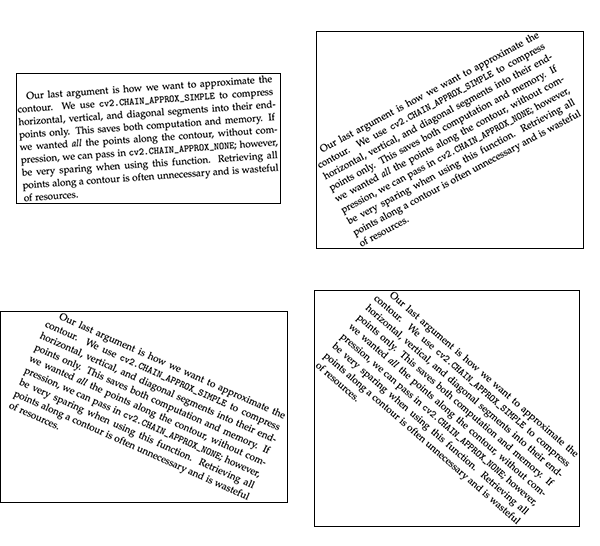
\includegraphics[width=3cm]{res/segment_text1.png}
    \caption{Good result on pure text}
  \end{subfigure}
  \hspace{5mm}%
  \begin{subfigure}[t]{4cm}
    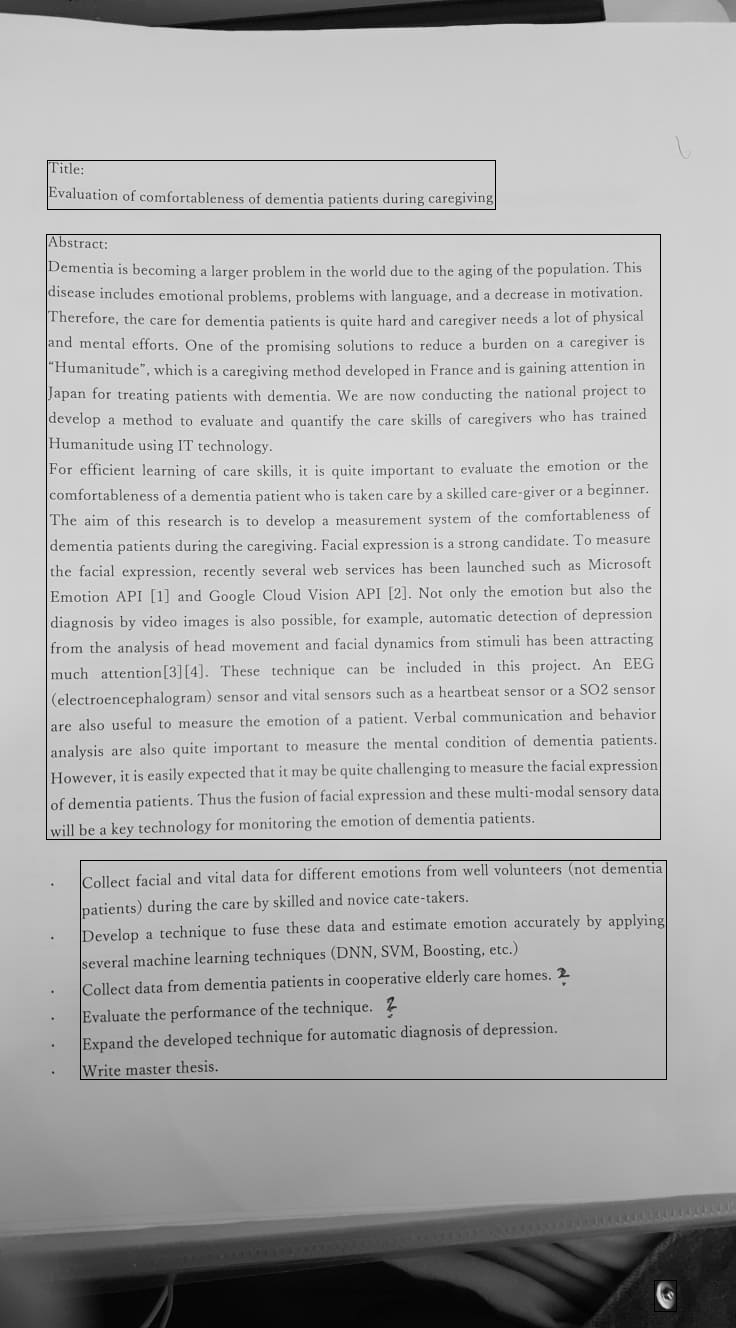
\includegraphics[width=3cm]{res/segment_text2.png}
    \caption{Good result on text on paper with little background noise}
  \end{subfigure}
  \hspace{5mm}%
  \begin{subfigure}[t]{4cm}
    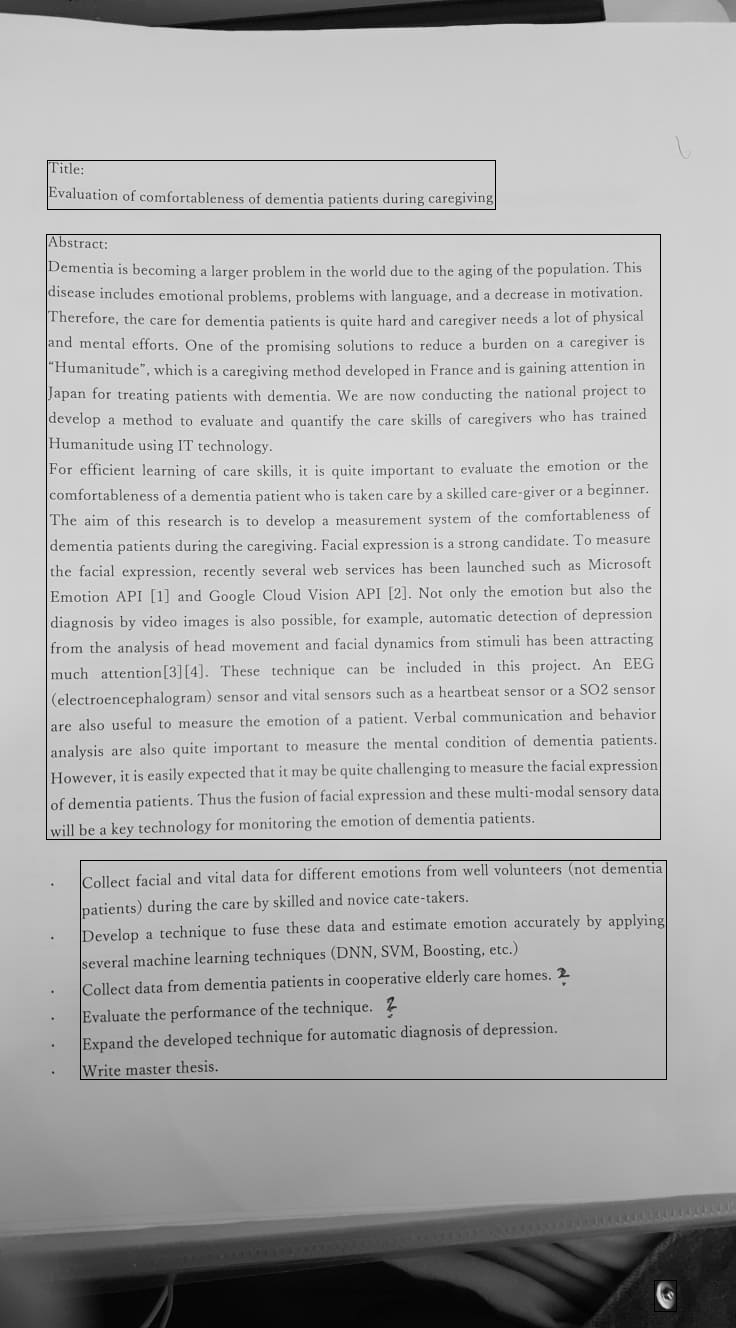
\includegraphics[width=3cm]{res/segment_text3.png}
    \caption{Bad result with many non text object segmented as text}
  \end{subfigure}
  \caption{Result of the Segment Text}
  \label{fig:Text_detection_result}
\end{figure}

\section{Result: Preprocessing}

\subsection{Rotation}
\begin{figure}[H]
  \centering
  
\includegraphics[height=4cm]{res/4angle_rot.png}
  \caption{cv.minAreaRect cannot differentiate between 0\textdegree and 180\textdegree, and 90\textdegree and 270\textdegree}
  \label{fig:4angle_rot}
\end{figure}


\subsection{Line segmentation}
\subsection{Character segmentation}
\section{Result: Classification}
\subsection{Description}
\begin{flushleft}
  Convolutional neural networks are especially good for image
  classification, because they take local spatial connections into account when
  they classify. This way it doesn't matter where in the image our
  object/character is it will be able to recognize it, same yields for rotation,
  as the CNN classifies based on local spatial connections it doesn't matter if
  the object is rotated. Hence the classification would be even more robust
  compared to the MLP.
\end{flushleft}

\section{Result: Datasets}
\subsection{Description}


\end{document}
